% Simple CMOS (N-MOSFET & P-MOSFET) H bridge.
% Author: Uli Koehler (https://techoverflow.net)
% Based on http://texample.net/tikz/examples/power-electronics-converter-inverter/
%
% NOTE: Requires recent CircuiTikZ version in order to use elmech and fetbodydiodes!
% TeXLive 2015 is too old, please use at least TeXLive 2016!
% 
\documentclass[tikz, border=1mm]{standalone}
\usepackage{siunitx}
\usepackage[european,cuteinductors,fetbodydiode]{circuitikz}

\usetikzlibrary{calc}
\ctikzset{bipoles/thickness=1}
\ctikzset{bipoles/length=0.8cm}
\ctikzset{bipoles/vsourceam/height/.initial=.7}
\ctikzset{bipoles/vsourceam/width/.initial=.7}
\tikzstyle{every node}=[font=\small]
\tikzstyle{every path}=[line width=0.8pt,line cap=round,line join=round]

\begin{document}
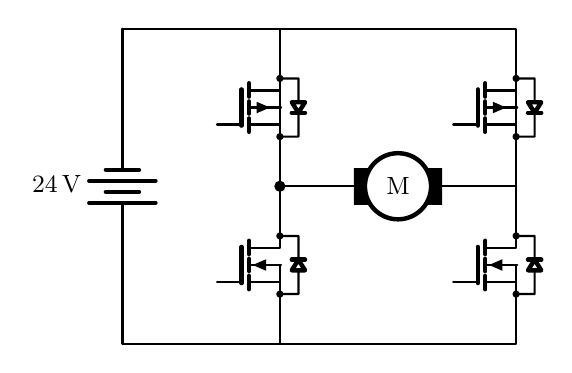
\begin{tikzpicture}
    \draw
    % DC source
    (0,0)
        to[battery, l=\SI{24}{\volt}] ++(0,4) coordinate (Vcc)
    ++(2,0) coordinate (NE)

    % Switches and diodes for left leg
    ++(0,-1) node [pigfete,scale=0.8,yscale=-1,name=fet1] {}
    ++(0,-2) node [nigfete,scale=0.8,name=fet4] {}
    (Vcc) -| (fet1.S)
    (fet1.D) -- (fet4.D)
    (fet4.S) |- (0,0)


    % Switches and diodes for leg b
    (NE)++(3,0)
    ++(0,-1) node [pigfete,scale=0.8,yscale=-1,name=fet3] {}
    ++(0,-2) node [nigfete,scale=0.8,name=fet2] {}
    %(fet3.D)++(0,0.1) -- ++(0.3,0) to[D*] ($(fet3.S)+(0.3,-0.1)$)
    %  -- ++(-0.3,0)
    %(fet2.S)++(0,0.1) -- ++(0.3,0) to[D*] ($(fet2.D)+(0.3,-0.1)$)
    %  -- ++(-0.3,0)
    % --Switch connections for leg b
    (Vcc) -| (fet3.S)
    (fet3.D) -- (fet2.D)
    (fet2.S) |- (0,0)

    % Motor (between the legs)
    (2,2) to[short,*-,current/distance=0.9,Telmech=M] ++(3,0)
    ;
\end{tikzpicture}
\end{document}